\chapter{Aromaticidade e substituição eletrofílica aromática}\label{ch:b2:aromatic-substitution}

A água de bromo perde a cor em segundos quando agitada com um alceno, e não a
perde de modo algum com o benzeno. No entanto, o benzeno reage com o bromo
assim que se adiciona um pouco de brometo de ferro(III) --- e o produto, o
bromobenzeno, ainda tem seu anel \omterm{def:b2:huckel:aromatic}{aromático} de seis membros: um hidrogênio foi
substituído, nada foi adicionado. Os anéis \omterm{def:b2:huckel:aromatic}{aromáticos} sofrem substituição, e
não adição, porque a adição jogaria fora a estabilização calculada no
\cref{ch:b2:huckel}. O mesmo mecanismo nitra, sulfona, alquila e acila os anéis
benzênicos, e os grupos já presentes em um anel decidem, com surpreendente
regularidade, aonde vai o próximo.

\begin{recall}
\Cref{ch:b2:huckel}: a aromaticidade e a \omterm{def:b2:huckel:delocalisation}{energia de deslocalização} do benzeno. O
volume do 1.º ano: adições eletrofílicas aos alcenos, efeitos indutivo e
mesomérico, grupos doadores e aceptores, carbocátions e seus rearranjos, o
postulado de Hammond, ácidos de Lewis, perfis de energia.
\end{recall}

\begin{omfigure}
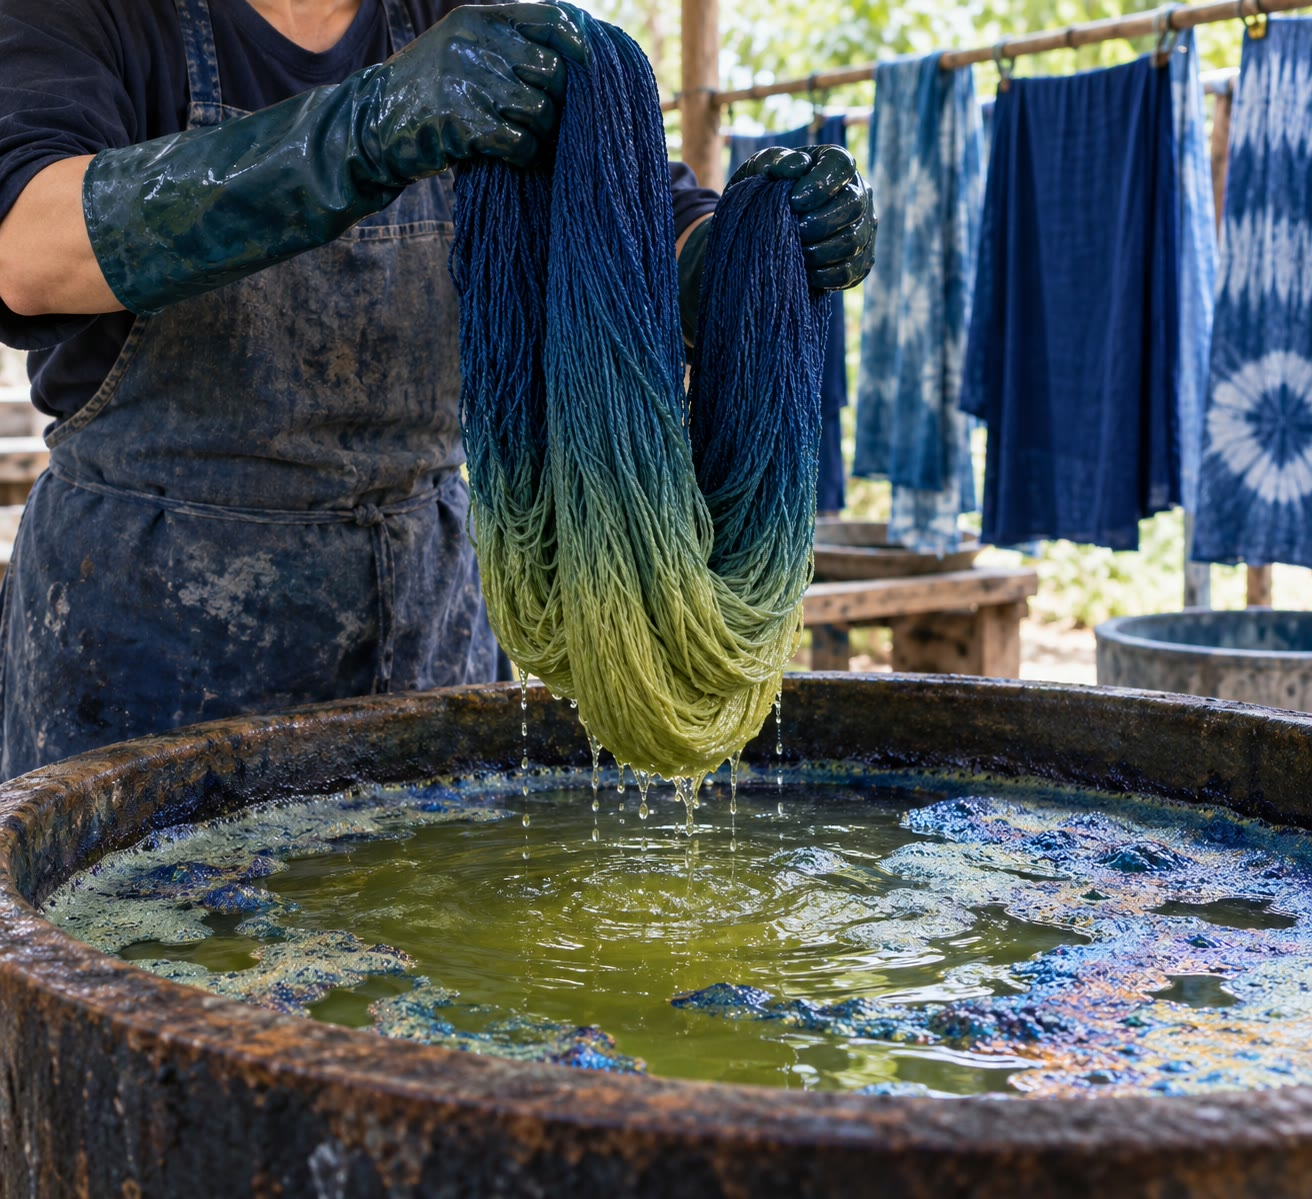
\includegraphics[width=0.55\linewidth]{images/book3/ai/b2-22-indigo-vat-2.jpg}

{\small Tingimento de fios em uma cuba de índigo (ilustração). O fio sai da
cuba amarelo-esverdeado, impregnado da forma reduzida solúvel do corante, e
fica azul ao ar, quando o oxigênio a transforma de volta em índigo insolúvel.
O índigo, como a maioria dos corantes, é construído sobre anéis \omterm{def:b2:huckel:aromatic}{aromáticos}; a
indústria de corantes do século XIX nasceu das reações de substituição deste
capítulo aplicadas ao benzeno do alcatrão de hulha.}
\end{omfigure}

\section{Substituição, e não adição}

\begin{definition}[Areno]\label{def:b2:aromatic-substitution:arene}
Um \emph{areno}\index{areno} é um hidrocarboneto que contém pelo menos um anel
\omterm{def:b2:huckel:aromatic}{aromático}, como o benzeno, o tolueno (metilbenzeno) ou o naftaleno; um grupo
arila (\ce{Ar}) é um areno menos um hidrogênio.
\end{definition}

\begin{proposition}[Por que o benzeno não sofre adição]\label{prop:b2:aromatic-substitution:no-addition}
Uma adição ao benzeno transformaria o anel \omterm{def:b2:huckel:aromatic}{aromático} em um ciclo-hexadieno não
\omterm{def:b2:huckel:aromatic}{aromático} e perderia a maior parte dos \qty{150}{kJ/mol} de estabilização
\omterm{def:b2:huckel:aromatic}{aromática}; a substituição a conserva.
\end{proposition}

\begin{proof}[Raciocínio]
No \cref{ch:b2:huckel}, a hidrogenação do benzeno a ciclo-hexa-1,3-dieno se
mostrou \omterm{def:b2:reaction-enthalpy:exothermic}{endotérmica} (\qty{+22}{kJ/mol}, a partir de \qty{-206.0}{} e
\qty{-227.7}{kJ/mol}), enquanto a de uma ligação dupla comum libera
\qty{119}{kJ/mol}: a primeira adição é a etapa custosa. Depois da primeira
etapa eletrofílica, o cátion formado pode adicionar um nucleófilo, o que deixa
um \omterm{def:b2:frontier-orbitals:diels-alder}{dieno} não \omterm{def:b2:huckel:aromatic}{aromático}, ou perder um próton, o que restaura o anel \omterm{def:b2:huckel:aromatic}{aromático}. O
segundo caminho é muito mais favorável.
% ledger: dfh:C6H6_g, dfh:C6H8_g, dfh:C6H10_g, dfh:C6H12_g
\end{proof}

\section{O mecanismo}

\begin{definition}[Substituição eletrofílica aromática]\label{def:b2:aromatic-substitution:seAr}
Uma \emph{substituição eletrofílica aromática}\index{substituicao eletrofilica aromatica@substituição eletrofílica aromática}
substitui um hidrogênio de um anel \omterm{def:b2:huckel:aromatic}{aromático} por um eletrófilo \ce{E+}. O
eletrófilo primeiro se liga a um carbono do anel, dando um cátion no qual esse
carbono é tetraédrico e a carga positiva está distribuída sobre os outros
cinco: o \emph{intermediário de Wheland}\index{intermediario de Wheland@intermediário de Wheland}
(um íon arênio). Uma base retira então o próton do carbono tetraédrico.
\end{definition}

\begin{proposition}[Duas etapas]\label{prop:b2:aromatic-substitution:mechanism}
A primeira etapa, que destrói a aromaticidade, é a lenta; a perda do próton,
que a restaura, é rápida.
\end{proposition}

\begin{proof}[Raciocínio]
O \omterm{def:b2:aromatic-substitution:seAr}{intermediário de Wheland} é um carbocátion estabilizado por deslocalização
sobre três carbonos, mas não \omterm{def:b2:huckel:aromatic}{aromático}: ele fica muito acima dos reagentes, e,
pelo postulado de Hammond, o estado de transição que leva a ele é próximo dele
em estrutura e em energia. A segunda etapa desce para um produto \omterm{def:b2:huckel:aromatic}{aromático}: sua
barreira é baixa.
\end{proof}

\begin{omfigure}
\begin{tikzpicture}
\begin{axis}[width=0.55\linewidth, height=5.4cm, xmin=-0.2, xmax=4.2, ymin=-5.5, ymax=11.5,
  axis x line=bottom, axis y line=left, xtick=\empty, ytick=\empty,
  xlabel={coordenada de reação}, ylabel={energia}, label style={font=\small}, clip=false]
\addplot[omDef, thick] table[x=x, y=sub] {figdata/out/bachelor-2-aromatic-profile.dat};
\addplot[omThm, thick, dashed, restrict x to domain=2:4] table[x=x, y=add] {figdata/out/bachelor-2-aromatic-profile.dat};
\node[font=\scriptsize, anchor=north west] at (axis cs:0.0,-0.6) {\ce{ArH + E+}};
\node[font=\scriptsize, anchor=north] at (axis cs:2,5.7) {Wheland};
\node[font=\scriptsize, anchor=west, omDef] at (axis cs:4.05,-4.0) {\ce{ArE + H+}};
\node[font=\scriptsize, anchor=west, omThm] at (axis cs:4.05,2.0) {produto de adição};
\node[font=\scriptsize, anchor=south] at (axis cs:1,10.1) {lenta};
\end{axis}
\end{tikzpicture}

{\small Perfil de energia de uma \omterm{def:b2:aromatic-substitution:seAr}{substituição eletrofílica aromática},
esquemático (um modelo). A primeira etapa, que forma o \omterm{def:b2:aromatic-substitution:seAr}{intermediário de
Wheland}, tem a barreira mais alta. A perda de um próton (contínua) restaura o
anel \omterm{def:b2:huckel:aromatic}{aromático}; a adição de um nucleófilo (tracejada) deixaria um produto
acima dos reagentes.}
\end{omfigure}

\begin{omfigure}
\setchemfig{atom sep=2em}
\schemestart
\chemfig{HO-\chemabove{N}{\scriptstyle +}(=[1]O)-[7]\chemabove{O}{\scriptstyle -}} \+ \chemfig{H_2SO_4}
\arrow{<=>}
\chemfig{O=N^{+}=O} \+ \chemfig{HSO_4^{-}} \+ \chemfig{H_2O}
\schemestop

\medskip
\begin{tikzpicture}[font=\small, >={Stealth}]
\tikzset{pics/whel/.style n args={4}{code={
    \foreach \k in {0,...,5} \draw[thick] ({90+60*\k}:0.7) -- ({150+60*\k}:0.7);
    \foreach \k in {#1} \draw[thick] ($({90+60*\k}:0.56)!0.18!({150+60*\k}:0.56)$) -- ($({90+60*\k}:0.56)!0.82!({150+60*\k}:0.56)$);
    \ifnum#2>-1 \node[font=\scriptsize] at ({90+60*#2}:0.36) {$+$};\fi
    \draw[thick] (270:0.7) -- ++(-125:0.42) node[anchor=north east, inner sep=1pt, font=\scriptsize] {H};
    \draw[thick] (270:0.7) -- ++(-55:0.42) node[anchor=north west, inner sep=1pt, font=\scriptsize] {#4};
    \if\relax\detokenize{#3}\relax\else
      \draw[thick] (90:0.7) -- (90:1.1) node[anchor=south, inner sep=1pt, font=\scriptsize] {#3};\fi
  }}}
  \foreach \k in {0,...,5} \draw[thick] ({90+60*\k}:0.7) -- ({150+60*\k}:0.7);
  \foreach \k in {0,2,4} \draw[thick] ($({90+60*\k}:0.56)!0.18!({150+60*\k}:0.56)$) -- ($({90+60*\k}:0.56)!0.82!({150+60*\k}:0.56)$);
  \node at (1.3,0) {$+$};
  \node at (2.0,0) {\ce{NO2+}};
  \draw[->, thick] (2.6,0) -- (3.8,0) node[midway, above, font=\scriptsize] {lenta};
  \pic at (4.7,0.1) {whel={1,4}{0}{}{\ce{NO2}}};
  \draw[->, thick] (5.6,0) -- (6.8,0) node[midway, above, font=\scriptsize] {rápida} node[midway, below, font=\scriptsize] {$-$\ce{H+}};
  \begin{scope}[xshift=7.7cm]
    \foreach \k in {0,...,5} \draw[thick] ({90+60*\k}:0.7) -- ({150+60*\k}:0.7);
    \foreach \k in {0,2,4} \draw[thick] ($({90+60*\k}:0.56)!0.18!({150+60*\k}:0.56)$) -- ($({90+60*\k}:0.56)!0.82!({150+60*\k}:0.56)$);
    \draw[thick] (270:0.7) -- (270:1.1) node[anchor=north, font=\scriptsize] {\ce{NO2}};
  \end{scope}
\end{tikzpicture}
\par\vspace{6pt}

{\small Nitração do benzeno. O ácido sulfúrico protona o ácido nítrico, que
perde água: o íon nitrônio \ce{NO2+} é o eletrófilo. Ele se liga a um carbono
(lenta), dando o \omterm{def:b2:aromatic-substitution:seAr}{intermediário de Wheland}, cuja carga positiva se distribui
pelo anel; a perda de um próton (rápida) dá o nitrobenzeno.}
\end{omfigure}

\section{As reações}

\paragraph{Halogenação.} O bromo ou o cloro sozinhos são eletrófilos fracos
demais; um ácido de Lewis (\ce{FeBr3}, \ce{AlCl3}) polariza o halogênio ao se
ligar a um de seus átomos, e o bromo externo ataca o anel.

\paragraph{Nitração.} Uma mistura de ácidos nítrico e sulfúrico concentrados
(acima) dá o íon nitrônio.

\paragraph{Sulfonação.} O ácido sulfúrico fumegante (\ce{SO3} em \ce{H2SO4})
dá o ácido benzenossulfônico. A reação é reversível: aquecer o ácido sulfônico
em ácido aquoso diluído remove de novo o grupo \ce{SO3H}, o que faz dele um
útil grupo bloqueador temporário.

\begin{definition}[Reações de Friedel--Crafts]\label{def:b2:aromatic-substitution:friedel-crafts}
Uma \emph{alquilação de Friedel--Crafts}\index{alquilacao de Friedel--Crafts@alquilação de Friedel--Crafts} liga um grupo
alquila a um anel \omterm{def:b2:huckel:aromatic}{aromático} a partir de um haloalcano e de um ácido de Lewis
(\ce{AlCl3}). Uma \emph{acilação de Friedel--Crafts}\index{acilacao de Friedel--Crafts@acilação de Friedel--Crafts}
liga um grupo acila \ce{RCO} a partir de um cloreto de acila e de \ce{AlCl3}, por
meio do \emph{íon acílio}\index{ion acilio@íon acílio} \ce{R-C#O+}, dando uma cetona arílica.
\end{definition}

\begin{proposition}[Limites das reações de Friedel--Crafts]\label{prop:b2:aromatic-substitution:friedel-crafts-limits}
A \omterm{def:b2:aromatic-substitution:friedel-crafts}{alquilação de Friedel--Crafts} sofre com os rearranjos do carbocátion e com a
polialquilação; a acilação para após uma substituição, não dá rearranjo e
exige pelo menos um equivalente de \ce{AlCl3}. Nenhuma das duas funciona em um
anel que tenha um grupo fortemente desativante.
\end{proposition}

\begin{proof}[Raciocínio]
O eletrófilo alquilante é um carbocátion (ou um complexo polarizado que se
comporta como tal), que se rearranja em outro mais estável por migrações de
hidreto ou de alquila: o 1-cloropropano dá sobretudo isopropilbenzeno. Um grupo
alquila ativa o anel (próxima seção); assim o produto reage mais depressa que
o benzeno e é alquilado de novo. O \omterm{def:b2:aromatic-substitution:friedel-crafts}{íon acílio} é estabilizado por ressonância
(\ce{R-C+=O} $\leftrightarrow$ \ce{R-C#O+}) e não se rearranja; o grupo acila
desativa o anel, de modo que o produto não reage mais; e a cetona formada liga
o \ce{AlCl3} por seu oxigênio, retirando o catalisador da reação: um
equivalente é consumido. Um anel fortemente desativado é um nucleófilo pobre
demais para esses eletrófilos fracos.
\end{proof}

\section{Efeitos dos substituintes}

\begin{definition}[Grupos orientadores]\label{def:b2:aromatic-substitution:directing}
Um substituinte em um anel benzênico é um \emph{grupo ativante}\index{grupo ativante} se o
anel reage mais depressa que o benzeno, e um \emph{grupo desativante}\index{grupo desativante}
se reage mais lentamente. Ele é um \emph{orientador orto/para}\index{orientador orto/para} se
o novo grupo entra principalmente nas posições vizinhas a ele e na oposta, e um
\emph{orientador meta}\index{orientador meta} se entra principalmente nas posições
seguintes a estas.
\end{definition}

\begin{proposition}[Doadores e aceptores]\label{prop:b2:aromatic-substitution:directing}
Os grupos que doam elétrons ao anel por efeito mesomérico (\ce{-OH}, \ce{-OCH3},
\ce{-NH2}, \ce{-NHCOCH3}) ou por efeito indutivo e \omterm{def:b2:fragment-orbitals:hyperconjugation}{hiperconjugação} (alquilas)
ativam o anel e orientam para orto/para. Os grupos que retiram elétrons por
efeito mesomérico (\ce{-NO2}, \ce{-CN}, \ce{-COR}, \ce{-COOH}, \ce{-SO3H}) o
desativam e orientam para meta.
\end{proposition}

\begin{proof}
Compare os \omterm{def:b2:aromatic-substitution:seAr}{intermediários de Wheland}. Para um ataque em orto ou em para de um
substituinte G, uma das três estruturas de ressonância coloca a carga positiva
no carbono que leva G; para um ataque em meta, nenhuma. Um G doador (um par não
ligante em O ou N) estabiliza uma carga positiva no carbono ao qual está
ligado, acrescentando uma quarta estrutura de ressonância em que todo átomo
tem um octeto: os intermediários orto e para são abaixados e, pelo postulado
de Hammond, também os estados de transição que levam a eles. Um G aceptor
desestabiliza uma carga positiva em seu carbono: os intermediários orto e para
são elevados, e o ataque em meta, que evita essa estrutura, é o menos
desfavorecido, embora mais lento que no benzeno.
\end{proof}

\begin{omfigure}
\begin{tikzpicture}[font=\small]
\tikzset{pics/whel/.style n args={4}{code={
    \foreach \k in {0,...,5} \draw[thick] ({90+60*\k}:0.7) -- ({150+60*\k}:0.7);
    \foreach \k in {#1} \draw[thick] ($({90+60*\k}:0.56)!0.18!({150+60*\k}:0.56)$) -- ($({90+60*\k}:0.56)!0.82!({150+60*\k}:0.56)$);
    \ifnum#2>-1 \node[font=\scriptsize] at ({90+60*#2}:0.36) {$+$};\fi
    \draw[thick] (270:0.7) -- ++(-125:0.42) node[anchor=north east, inner sep=1pt, font=\scriptsize] {H};
    \draw[thick] (270:0.7) -- ++(-55:0.42) node[anchor=north west, inner sep=1pt, font=\scriptsize] {#4};
    \if\relax\detokenize{#3}\relax\else
      \draw[thick] (90:0.7) -- (90:1.1) node[anchor=south, inner sep=1pt, font=\scriptsize] {#3};\fi
  }}}
  \node[anchor=east] at (-1.0,0) {metoxila, ataque em para:};
  \pic at (0,0) {whel={1,4}{0}{\ce{OCH3}}{E}};
  \node at (1.25,0.1) {$\leftrightarrow$};
  \begin{scope}[xshift=2.5cm]
    \foreach \k in {0,...,5} \draw[thick] ({90+60*\k}:0.7) -- ({150+60*\k}:0.7);
    \foreach \k in {1,4} \draw[thick] ($({90+60*\k}:0.56)!0.18!({150+60*\k}:0.56)$) -- ($({90+60*\k}:0.56)!0.82!({150+60*\k}:0.56)$);
    \draw[thick] (-0.06,0.7) -- (-0.06,1.1); \draw[thick] (0.06,0.7) -- (0.06,1.1);
    \node[anchor=south, inner sep=1pt, font=\scriptsize] at (0,1.1) {$\overset{+}{\mathrm O}\mathrm{CH_3}$};
    \draw[thick] (270:0.7) -- ++(-125:0.42) node[anchor=north east, inner sep=1pt, font=\scriptsize] {H};
    \draw[thick] (270:0.7) -- ++(-55:0.42) node[anchor=north west, inner sep=1pt, font=\scriptsize] {E};
  \end{scope}
  \node[anchor=west, font=\scriptsize] at (3.4,0) {estrutura adicional, todos os átomos com octeto};
  \begin{scope}[yshift=-3.5cm]
    \node[anchor=east] at (-1.0,0) {nitro, ataque em para:};
    \pic at (0,0) {whel={1,4}{0}{\ce{NO2}}{E}};
    \node[anchor=west, font=\scriptsize] at (1.0,0) {carga positiva no carbono que leva o aceptor};
  \end{scope}
\end{tikzpicture}

{\small \omterm{def:b2:aromatic-substitution:seAr}{Intermediários de Wheland} para um ataque em para de um substituinte.
Com a metoxila, um par não ligante do oxigênio compartilha a carga positiva
(uma estrutura de ressonância adicional, todos os átomos com octeto): o
intermediário é estabilizado, e o substituinte é ativante e \omterm{def:b2:aromatic-substitution:directing}{orientador
orto/para}. Com o nitro, uma estrutura coloca a carga positiva no carbono que
leva o grupo retirador de elétrons: o intermediário é desestabilizado, e o
ataque ocorre em meta.}
\end{omfigure}

\begin{proposition}[Os halogênios]\label{prop:b2:aromatic-substitution:halogens}
Os substituintes halogênio desativam o anel, mas orientam para orto/para.
\end{proposition}

\begin{proof}[Raciocínio]
Sua retirada indutiva (eletronegatividade) diminui a densidade eletrônica do
anel inteiro e desacelera todo ataque: desativante. Mas um par não ligante do
halogênio ainda pode compartilhar a carga positiva dos \omterm{def:b2:aromatic-substitution:seAr}{intermediários de
Wheland} orto e para, o que o intermediário meta não pode aproveitar: entre os
ataques mais lentos, orto e para continuam sendo os menos lentos.
\end{proof}

\section{Benzenos polissubstituídos}

\begin{method}[Prever a posição da substituição]\label{met:b2:aromatic-substitution:predict-position}
\begin{enumerate}
  \item Para cada substituinte, marque as posições que ele favorece (orto/para
        ou meta).
  \item Se eles concordam, essa posição vence. Se discordam, decide o ativante
        mais forte (\ce{-NH2}, \ce{-OH} $>$ \ce{-OCH3} $>$ \ce{-NHCOCH3} $>$ alquila $>$ halogênio).
  \item Evite a posição entre dois substituintes em relação 1,3 (impedida) e
        espere para em vez de orto quando os grupos forem volumosos.
\end{enumerate}
\end{method}

\begin{method}[Planejar uma síntese aromática]\label{met:b2:aromatic-substitution:plan-aromatic}
\begin{enumerate}
  \item Escolha a ordem das etapas de modo que cada grupo já presente oriente o
        seguinte para onde ele é desejado: para fazer o 3-bromonitrobenzeno,
        nitre primeiro (\omterm{def:b2:aromatic-substitution:directing}{orientador meta}) e depois bromo; para fazer o
        4-bromonitrobenzeno, bromo primeiro.
  \item Use grupos conversíveis: um grupo acila (meta) pode ser reduzido a
        alquila (orto/para); um grupo nitro (meta), reduzido a amina
        (orto/para); uma alquila, oxidada a \ce{-COOH} (meta).
  \item Bloqueie uma posição com \ce{-SO3H} e remova-o no final.
  \item Dome um ativante forte: uma amina é acilada (\ce{-NHCOCH3}) antes da
        nitração ou da halogenação e depois liberada de novo.
\end{enumerate}
\end{method}

\begin{history}[Friedel e Crafts]
\begin{minipage}[t]{0.18\linewidth}
\vspace{0pt}
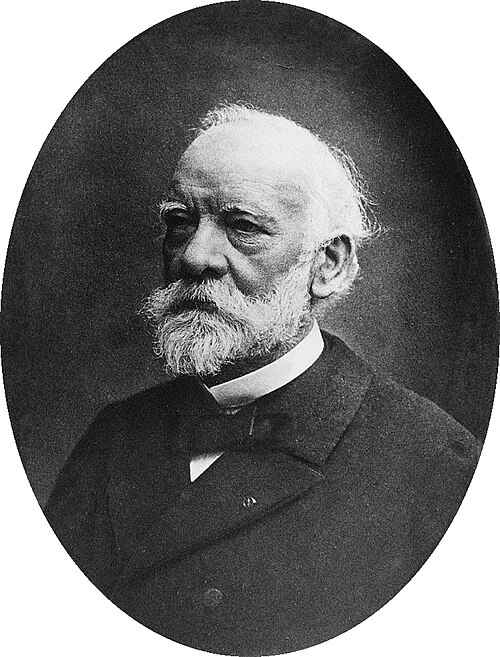
\includegraphics[width=\linewidth]{images/book3/friedel.jpg}
\end{minipage}\hspace{0.02\linewidth}%
\begin{minipage}[t]{0.18\linewidth}
\vspace{0pt}
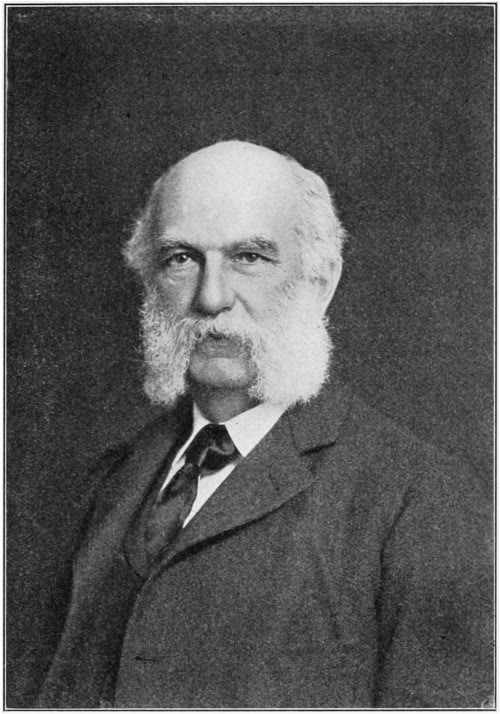
\includegraphics[width=\linewidth]{images/book3/crafts.jpg}
\end{minipage}\hfill
\begin{minipage}[t]{0.58\linewidth}
\vspace{0pt}
Em 1877, Charles Friedel e James Mason Crafts, trabalhando juntos em Paris,
descobriram que o cloreto de alumínio faz os haloalcanos e os cloretos de
acila reagirem com o benzeno. Suas reações se tornaram o modo padrão de ligar
grupos carbonados a anéis \omterm{def:b2:huckel:aromatic}{aromáticos}, e a catálise por ácidos de Lewis que eles
descobriram foi muito além delas. (Retratos: Friedel, década de 1890; Crafts,
da \textit{Popular Science Monthly}, 1900; domínio público, Wikimedia Commons.)
\end{minipage}
\end{history}

\begin{safety}{\ghs[5mm]{GHS02}\,\ghs[5mm]{GHS05}\,\ghs[5mm]{GHS06}\,\ghs[5mm]{GHS08}}
O benzeno é cancerígeno e é substituído pelo tolueno ou por outros \omterm{def:b2:aromatic-substitution:arene}{arenos}
sempre que possível. Os ácidos nítrico e sulfúrico concentrados são corrosivos
e a mistura nitrante é fortemente oxidante; ela é resfriada e o \omterm{def:b2:aromatic-substitution:arene}{areno} é
adicionado lentamente, pois as nitrações são \omterm{def:b2:reaction-enthalpy:exothermic}{exotérmicas}. O bromo é muito
tóxico e corrosivo; o cloreto de alumínio reage violentamente com a água. Os
nitroarenos são tóxicos.
% ledger: ghs:benzene, ghs:toluene, ghs:HNO3, ghs:H2SO4, ghs:Br2, ghs:AlCl3, ghs:nitrotoluene-4
\end{safety}

\section{Exercícios}

\begin{exercise}[$\star$]\label{exo:b2:aromatic-substitution:1}
Escreva a formação do íon nitrônio a partir do ácido nítrico e do ácido sulfúrico.
\end{exercise}

\begin{exercise}[$\star$]\label{exo:b2:aromatic-substitution:2}
Dê os produtos principais da bromação (\ce{Br2}, \ce{FeBr3}) do tolueno e do
nitrobenzeno.
\end{exercise}

\begin{exercise}[$\star$]\label{exo:b2:aromatic-substitution:3}
Classifique como ativante ou desativante, orto/para ou meta: \ce{-CH3}, \ce{-OH}, \ce{-Cl},
\ce{-NO2}, \ce{-COCH3}, \ce{-NHCOCH3}.
\end{exercise}

\begin{exercise}[$\star$]\label{exo:b2:aromatic-substitution:4}
Dê o produto do benzeno com cloreto de etanoíla e cloreto de alumínio.
\end{exercise}

\begin{exercise}[$\star\star$]\label{exo:b2:aromatic-substitution:5}
O benzeno e o 1-cloropropano com \ce{AlCl3} dão sobretudo isopropilbenzeno.
Explique e dê uma via em duas etapas até o propilbenzeno.
\end{exercise}

\begin{exercise}[$\star\star$]\label{exo:b2:aromatic-substitution:6}
O fenol descora a água de bromo de imediato, sem catalisador, dando o
2,4,6-tribromofenol. Explique.
\end{exercise}

\begin{exercise}[$\star\star$]\label{exo:b2:aromatic-substitution:7}
Dê sínteses do 3-bromonitrobenzeno e do 4-bromonitrobenzeno a partir do benzeno.
\end{exercise}

\begin{exercise}[$\star\star$]\label{exo:b2:aromatic-substitution:8}
A anilina é mal nitrada (oxidação e produto meta), mas a acetanilida dá
sobretudo 4-nitroacetanilida. Explique os dois fatos.
\end{exercise}

\begin{exercise}[$\star\star$]\label{exo:b2:aromatic-substitution:9}
Mostre como um grupo ácido sulfônico pode ser usado para preparar o 2-bromotolueno isento de seu isômero para.
\end{exercise}

\begin{exercise}[$\star\star\star$]\label{exo:b2:aromatic-substitution:10}
Onde o 4-metilanisol (4-metoxitolueno) sofre nitração? Explique com os dois
grupos orientadores.
\end{exercise}

\begin{exercise}[$\star\star\star$]\label{exo:b2:aromatic-substitution:11}
O 2,4,6-trinitrotolueno é obtido por três nitrações sucessivas do tolueno,
cada uma em condições mais drásticas. Explique por quê.
\end{exercise}

\begin{exercise}[$\star\star\star$]\label{exo:b2:aromatic-substitution:12}
Proponha uma síntese do ácido 4-nitrobenzoico a partir do tolueno, e do ácido 3-nitrobenzoico.
\end{exercise}

\section{Problema: Nitrar o tolueno}

\begin{problem}[{Problema de fim de semana --- o íon nitrônio e o mecanismo da
nitração, as posições orto, meta e para do tolueno comparadas à razão
estatística, a separação dos isômeros e um balanço de massa}]
\label{pb:b2:aromatic-substitution:1}
Dados: pontos de fusão: 2-nitrotolueno \qty{-10}{\degreeCelsius}, 3-nitrotolueno
\qty{16}{\degreeCelsius}, 4-nitrotolueno \qty{52}{\degreeCelsius}. Dados do
exercício para um ensaio: \qty{100}{g} de tolueno, \omterm{def:b2:continuous-reactors:conversion}{conversão} de 90~\%,
distribuição dos isômeros 58~\% orto, 4~\% meta, 38~\% para. Massas molares
(\unit{g/mol}): C 12.011, H 1.008, N 14.007, O 15.999.
% ledger: mp:2-nitrotoluene, mp:3-nitrotoluene, mp:4-nitrotoluene, aw:C, aw:H, aw:N, aw:O

\medskip
\noindent\textbf{Parte I --- O eletrófilo e o mecanismo.}
\begin{enumerate}
  \item Escreva a formação do íon nitrônio.
  \item Desenhe sua estrutura de Lewis e dê sua forma.
  \item Escreva o ataque de \ce{NO2+} ao tolueno em para da metila.
  \item Desenhe as três estruturas de ressonância do \omterm{def:b2:aromatic-substitution:seAr}{intermediário de Wheland} para.
  \item Qual etapa é determinante da velocidade?
  \item O que retira o próton na segunda etapa?
\end{enumerate}

\medskip
\noindent\textbf{Parte II --- As três posições.}
\begin{enumerate}[resume]
  \item Quantas posições orto, meta e para tem o tolueno?
  \item Que razão daria um ataque ao acaso?
  \item Desenhe o \omterm{def:b2:aromatic-substitution:seAr}{intermediário de Wheland} meta e explique por que ele é o
        menos estabilizado.
  \item Como o grupo metila estabiliza os intermediários orto e para?
  \item Compare a razão observada com a estatística: quais posições são favorecidas?
  \item Compare o rendimento por posição em orto (metade da porcentagem orto)
        e em para. Sugira uma razão para a diferença.
  \item O tolueno é nitrado mais depressa ou mais lentamente que o benzeno?
\end{enumerate}

\medskip
\noindent\textbf{Parte III --- A separação.}
\begin{enumerate}[resume]
  \item Qual isômero é sólido à temperatura ambiente?
  \item Sugira como isolá-lo da mistura por resfriamento.
  \item Por que a simetria favorece um ponto de fusão alto?
  \item Como os isômeros orto e meta poderiam ser separados em seguida?
  \item Por que esses isômeros são difíceis de separar por destilação simples?
\end{enumerate}

\medskip
\noindent\textbf{Parte IV --- Balanço de massa.}
\begin{enumerate}[resume]
  \item Calcule a massa molar do tolueno e do nitrotolueno.
  \item Calcule a quantidade de tolueno e a de nitrotolueno formado.
  \item Calcule as massas dos três isômeros.
  \item Que reação posterior deve ser evitada resfriando e não usando excesso de ácido?
  \item Como você obteria o ácido 4-nitrobenzoico a partir do isômero para?
  \item Dê a massa de 4-nitrotolueno obtida a partir de \qty{100}{g} de tolueno nesse ensaio.
\end{enumerate}
\end{problem}
